\documentclass{article}
\usepackage[utf8]{inputenc}
\usepackage{graphicx}
\usepackage{hyperref}
\usepackage{geometry}
\geometry{a4paper} % Set the page size to A4
\usepackage{listings} % Package for including code in the document

\title{Práctica 07: Funciones en SQL}
\author{Carlos I. Padilla Herrera}
\date{13 de mayo de 2024}

\lstset{frame=single, % Adds a frame around the code
        basicstyle=\small\ttfamily, % Use a small, true type font
        language=SQL, % SQL syntax highlighting
        showstringspaces=false} % Don't mark spaces in strings

\begin{document}

\begin{titlepage}
    \centering
    \vspace*{1cm}
    \Huge\textbf{Curso de base de datos entre semana G0224}
    
    \vspace{0.5cm}
    \LARGE Escuela de Código PILARES
    
    \vspace{1.5cm}
    \textbf{Carlos Ignacio Padilla Herrera}
    
    \vspace{2cm}
    \Large\textbf{Folio:} 794DR02
    
    \vspace{0.5cm}
    \Large\textbf{Práctica 02:} Diseño de un modelo relacional.
    
    \vfill
    
    \Large\textbf{Fecha:} 13 de mayo de 2024.
    
    \vspace{0.8cm}
\end{titlepage}

\begin{figure}[ht]
    \centering
    {
        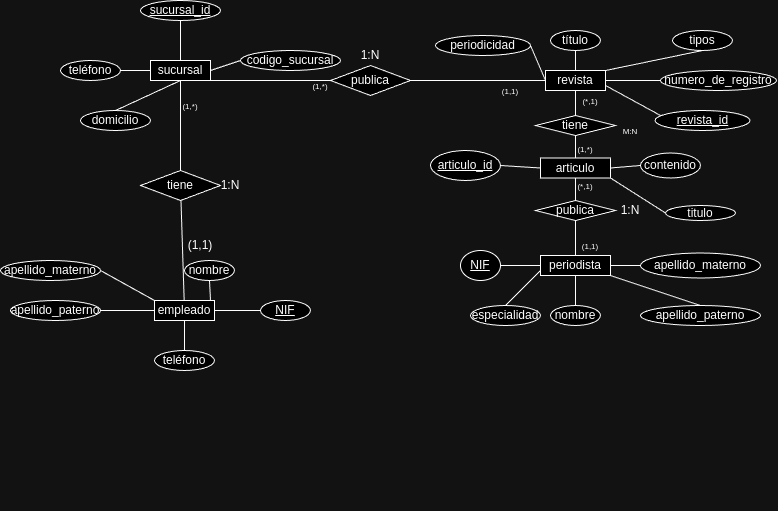
\includegraphics[width=\linewidth]{02practica.png} % Asegúrate de que el nombre del archivo y la extensión son correctos
    }
    \caption{Diseño del modelo relacional de la base de datos de proveedores.}
\end{figure}

\newpage


\end{document}
